\documentclass[12pt,a4paper]{article}

% Pakiety dla polskich znaków
\usepackage[utf8]{inputenc}
\usepackage[T1]{fontenc}
\usepackage[english]{babel}
\babelprovide[import]{polish}

% Pakiety matematyczne
\usepackage{amsmath}
\usepackage{amssymb}
\usepackage{amsfonts}

% Pakiety dla grafiki
\usepackage{graphicx}
\usepackage{float}
\usepackage{subcaption}

% Pakiety dla tabel
\usepackage{booktabs}
\usepackage{tabularx}
\usepackage{array}
\usepackage{multirow}
\usepackage{makecell}

% Pakiety dla lepszego formatowania
\usepackage{geometry}
\geometry{a4paper, margin=2.5cm}
\usepackage{setspace}
\onehalfspacing
\usepackage[expansion=false]{microtype}
\setlength{\emergencystretch}{1.5em}

% Pakiety dla hiperlinków i kolorów
\usepackage{xurl}
\usepackage{hyperref}
\hypersetup{
    colorlinks=true,
    linkcolor=blue,
    citecolor=blue,
    urlcolor=blue
}

% Pakiety dla lepszych list
\usepackage{enumitem}

% Informacje o dokumencie
\title{Adaptacyjne sterowanie sygnalizacją świetlną z wykorzystaniem PPO-Transformer i detekcji RFID w środowisku SUMO}
\author{Daniel Kleczyński \and Michał Kocik}
\date{\today}

\begin{document}
\selectlanguage{polish}

\maketitle

\begin{abstract}
W pracy przedstawiono metodę adaptacyjnego sterowania sygnalizacją świetlną opartą o algorytm Proximal Policy Optimization (PPO) zintegrowany z architekturą Transformer, wykorzystującą wyłącznie detekcję pojazdów opartą o technologię RFID w środowisku symulacyjnym SUMO. Czytniki RFID pełnią funkcję detektorów pojazdów, generując strumień zagregowanych zliczeń w krótkich oknach czasowych. Strumień ten jest modelowany sekwencyjnie przez Transformer, umożliwiając polityce PPO przechwycenie zmienności napływu pojazdów i podejmowanie decyzji o utrzymaniu lub zmianie fazy przy zachowaniu ograniczeń bezpieczeństwa. Funkcja nagrody została zaprojektowana w celu minimalizacji globalnego czasu podróży i długości kolejek. Eksperymentalnie porównano proponowaną metodę z klasycznym algorytmem sekwencyjnym oraz adaptacyjnym algorytmem Millera, wykorzystując identyczne dane wejściowe i ograniczenia fazowe. Analiza wrażliwości wykazuje odporność PPO-Transformer na częściowe utraty odczytów RFID oraz na zmienne natężenie ruchu.
\end{abstract}

\textbf{Słowa kluczowe:} PPO, Transformer, RFID, SUMO, RL, sterowanie sygnalizacja, TraCI

\section{Wstęp}

Dynamiczne zarządzanie ruchem miejskim wymaga algorytmów zdolnych do adaptacji do zmiennych potoków pojazdów. Klasyczne systemy o stałej sekwencji faz nie reagują na wahania natężenia i struktury ruchu. Rozwiązania oparte o uczenie ze wzmocnieniem (RL/DRL) stają się naturalnym kandydatem do sterowania sygnalizacją w czasie rzeczywistym, szczególnie gdy dysponujemy strumieniem wiarygodnych pomiarów z sensorów infrastruktury~\cite{ref1,ref2}. W tym projekcie kluczowym źródłem danych są czytniki RFID, które w sposób odporny na warunki pogodowe dostarczają informacji o typach pojazdów i ich pojawianiu się na wlotach skrzyżowania~\cite{ref3}.

Technologia RFID stanowi kluczowy komponent proponowanego systemu, zapewniając niezawodne i chroniące prywatność źródło danych dla algorytmów głębokiego uczenia ze wzmocnieniem (DRL). W przeciwieństwie do detekcji opartej na wizji, RFID jest odporna na niekorzystne warunki pogodowe (deszcz, mgła, śnieg), poprawiając niezawodność inteligentnych systemów transportowych (ITS)~\cite{ref3}. Agregując jedynie obecność pojazdów i ich typ, bez obrazów lub szczegółowych trajektorii, eliminuje typowe problemy związane z RODO, jednocześnie umożliwiając klasyfikację typów pojazdów (samochody osobowe, pojazdy ciężarowe, pojazdy uprzywilejowane) z dokładnością przekraczającą 95\%~\cite{ref3}. Agregowane pomiary RFID, przetwarzane w krótkich oknach czasowych, są dobrze dostosowane do sekwencyjnych modeli opartych na Transformer, które przechwytują wzorce przestrzenno-czasowe ruchu i określają sterowanie sygnalizacją.

\section{Przegląd systemu i architektura}

\subsection{Przepływ danych i sterowania (pętla zamknięta)}

Punktem wyjścia są zliczenia z detektorów RFID (E1) umieszczonych na każdym pasie wlotowym. Liczniki są agregowane w oknie czasowym i przekształcane do wektora obserwacji, który jest następnie składany w sekwencję długości $L$ i przekazywany do enkodera Transformer. Wyjście modelu stanowi decyzja o wyborze fazy oraz korekta czasu zielonego. Logika bezpieczeństwa wymusza minimalne i maksymalne czasy zielonego oraz fazę żółtą.

\begin{figure}[H]
\centering
\includegraphics[width=0.8\textwidth]{Rys/R1.png}
\caption{Koncepcja zamkniętej pętli sterowania: symulacja generuje kongestię, system detekcji (RFID) dostarcza dane wejściowe, a model wyznacza sygnały sterujące sygnalizacją.}
\label{fig:r1}
\end{figure}

\subsection{Geneza podejścia (platforma RFID → SUMO)}

Wcześniejsze prace nad sterowaniem opartym o RFID były prowadzone na makiecie skrzyżowania, gdzie czytniki RFID pełniły rolę detektorów i umożliwiały prostą adaptację sterowania. Jednak wraz ze wzrostem liczby skrzyżowań i różnorodności floty rośnie złożoność problemu (eksplozja przestrzeni stanów), co uzasadnia przejście do środowiska symulacyjnego i zastosowanie DRL.

\begin{figure}[H]
\centering
\includegraphics[width=0.7\textwidth]{Rys/R2.png}
\caption{Makieta skrzyżowania z systemem RFID -- rozmieszczenie czytników i stref odczytu.}
\label{fig:r2}
\end{figure}

\begin{figure}[H]
\centering
\includegraphics[width=0.7\textwidth]{Rys/R3.png}
\caption{Ilustracja eksplozji przestrzeni stanów w funkcji liczby skrzyżowań -- motywacja dla podejść uczących się.}
\label{fig:r3}
\end{figure}

\subsection{Opis scenariusza symulacyjnego}

Badania przeprowadzono na modelu izolowanego skrzyżowania czterowlotowego. Ta architektura jest powszechnie stosowana jako podstawowy scenariusz testowy dla nowych algorytmów sterowania sygnalizacją~\cite{ref1}. System działa w dwóch głównych, niekonfliktowych fazach: Faza 0 (nadanie priorytetu kierunkowi północ-południe, N$\leftrightarrow$S) oraz Faza 1 (nadanie priorytetu kierunkowi wschód-zachód, W$\leftrightarrow$E). W celu zapewnienia bezpieczeństwa i płynności ruchu wprowadzono twarde ograniczenia czasowe: minimalny czas trwania fazy zielonej ($t_{\text{green}}^{\text{min}} = 10$ s), maksymalny czas trwania fazy zielonej ($t_{\text{green}}^{\text{max}} = 60$ s), a także stały czas fazy żółtej (3 s) oraz interwał międzyzielony.

Wszystkie eksperymenty przeprowadzono przy użyciu mikroskopowego symulatora SUMO, wersja 1.19~\cite{ref4}. SUMO zostało wybrane jako platforma badawcza ze względu na szeroką akceptację w środowisku naukowym, wysoką wierność modelowania dynamiki pojazdów oraz elastyczne API (w tym sumo-rl), które umożliwia integrację z bibliotekami głębokiego uczenia. Model SUMO został skalibrowany zgodnie z wytycznymi FHWA (Federal Highway Administration) w celu zapewnienia realistycznej dynamiki ruchu~\cite{ref7}. Czytniki RFID (symulowane w SUMO jako detektory typu Induction Loop) umieszczone na każdym wlocie $j \in \{1,2,3,4\}$ zliczają pojazdy, rozróżniając trzy predefiniowane klasy: samochody osobowe, autobusy i karetki pogotowia.

\begin{figure}[H]
\centering
\includegraphics[width=0.8\textwidth]{Rys/R4.png}
\caption{Wizualizacja analizowanego skrzyżowania oraz koncepcja rozmieszczenia czytników RFID na wlotach.}
\label{fig:r4}
\end{figure}

\section{Podstawy teoretyczne}

\subsection{Definicja MDP}

Problem sterowania zdefiniowano jako MDP:
\begin{equation}
M = (S, A, P, R, \gamma)
\end{equation}
gdzie $S$ to przestrzeń stanów, $A$ to przestrzeń akcji, $P$ to przejścia, $R$ to nagroda, a $\gamma$ jest współczynnikiem dyskonta.

\subsection{Obserwacje i sekwencje}

Dla każdego wlotu $j \in \{1,2,3,4\}$ budowany jest wektor zliczeń pojazdów:
\begin{equation}
c_t^{(j)} = [n_{t,\text{car}}^{(j)}, n_{t,\text{bus}}^{(j)}, n_{t,\text{amb}}^{(j)}]
\end{equation}

Pełna obserwacja na kroku $t$ ma postać:
\begin{equation}
o_t = [c_t^{(1)} \Vert c_t^{(2)} \Vert c_t^{(3)} \Vert c_t^{(4)} \Vert p_t \Vert \tau_t]
\end{equation}
gdzie $p_t \in \{0,1\}^K$ to one-hot fazy ($K=2$), a $\tau_t$ to znormalizowany czas trwania aktualnej fazy:
\begin{equation}
\tau_t = \frac{g_t^{\text{elapsed}}}{g_{\text{max}}}
\end{equation}
W niniejszej implementacji $g_t^{\text{elapsed}}$ odpowiada \path{phase_elapsed}, a $g_{\text{max}}$ odpowiada $t_{\text{green\_max}}$.

Zgodnie z konwencją w artykule wzorcowym, obserwacja może być opisana również przez wymiar:
\begin{equation}
o_t \in \mathbb{R}^{12 + K + 1}
\end{equation}
tj. $12$ cech zliczeń (4 wloty $\times$ 3 klasy), $K=2$ cechy fazy oraz 1 cecha $\tau_t$.

Wejście do Transformer to sekwencja:
\begin{equation}
X_t = [o_{t-L+1}, \dots, o_t]
\end{equation}
oraz, analogicznie do równania (4) w artykule wzorcowym:
\begin{equation}
X_t \in \mathbb{R}^{L \times D}, \quad D = 12 + K + 1
\end{equation}

W implementacji $L=48$ i $\Delta t=5$ s, co odpowiada 4 minutom historii.

\subsection{Przestrzeń akcji i ograniczenia bezpieczeństwa}

Akcja jest dwu-wymiarowa:
\begin{equation}
a_t = (a_t^{\text{phase}}, a_t^{\text{dur}})
\end{equation}
gdzie $a_t^{\text{phase}} \in \{0,1\}$ (N-S lub E-W), a $a_t^{\text{dur}} \in \{-5, 0, +5\}$ sekund. Zmiana fazy jest dozwolona jedynie, gdy spełnione są ograniczenia:
\begin{equation}
t_{\text{green\_min}} \leq t_{\text{green}} \leq t_{\text{green\_max}}
\end{equation}
oraz uwzględniana jest faza żółta o czasie 3s.

\subsection{Funkcja nagrody}

Nagroda jest ujemna i łączy trzy kryteria:
\begin{equation}
r_t = - \alpha \cdot \text{delay}_t - \beta \cdot \text{queue}_t - \gamma \cdot \text{stops}_t
\end{equation}
Współczynniki z konfiguracji: $\alpha=0.55$, $\beta=0.30$, $\gamma=0.15$.
W odniesieniu do artykułu wzorcowego, $\text{delay}_t$, $\text{queue}_t$ i $\text{stops}_t$ odpowiadają odpowiednio: przyrostowi opóźnień (na podstawie waiting time), łącznej/uszeregowanej wielkości kolejki (zliczenia pojazdów zatrzymanych) oraz liczbie zdarzeń zatrzymania w oknie czasowym sterowania.

\subsection{PPO -- funkcja celu}

Stosujemy standardowy obcięty cel PPO:
\begin{equation}
L_{\text{CLIP}}(\theta) = \mathbb{E}_t \left[\min(r_t(\theta) \hat{A}_t, \text{clip}(r_t(\theta), 1-\epsilon, 1+\epsilon) \hat{A}_t)\right]
\end{equation}
gdzie $r_t(\theta) = \frac{\pi_\theta(a_t|s_t)}{\pi_{\theta_{\text{old}}}(a_t|s_t)}$.

\subsection{Model zakłóceń RFID}

Zakłócenia odczytów są modelowane poprzez losowe gubienie zliczeń:
\begin{equation}
\tilde{n}_t \sim \text{Binomial}(n_t, 1 - p_{\text{noise}})
\end{equation}
gdzie $p_{\text{noise}}$ odpowiada \path{rfid_noise_rate} (w eksperymencie 0.2).

\section{Metodyka}

\subsection{Architektura agenta: PPO-Transformer}

Do modelowania polityki sterowania zastosowano hybrydową architekturę łączącą algorytm PPO z enkoderem Transformer. Wybór algorytmu PPO był podyktowany jego wysoką stabilnością, efektywnością próbkowania oraz mniejszą wrażliwością na strojenie hiperparametrów w porównaniu z innymi metodami gradientu polityki~\cite{ref5}. Algorytm PPO stabilizuje trening poprzez ograniczenie aktualizacji polityki za pomocą obciętego celu, upraszczając podejście trust-region z TRPO przy jednoczesnym zmniejszeniu złożoności obliczeniowej~\cite{ref5}. Jest szeroko stosowany w sterowaniu wieloskrzyżowaniowym, skutecznie równoważąc eksplorację i eksploatację~\cite{ref2}.

Integralnym komponentem architektury jest moduł Transformer, wykorzystywany do efektywnego modelowania zależności czasowych w sekwencyjnych danych z transponderów RFID~\cite{ref6}. Mechanizm self-attention umożliwia ważenie znaczenia historycznych stanów ruchu, pozwalając na wykrywanie wzorców (np. kolumny pojazdów) i podejmowanie decyzji predykcyjnych.

Proces przygotowania danych wejściowych, wizualizowany na Rysunku~\ref{fig:r5}, obejmuje spłaszczenie informacji na poziomie pasów i ich konkatenację. Sekwencja wejściowa $X_t$ przekazywana do enkodera składa się z okna $L$ najnowszych obserwacji, zgodnie z równaniem (4). W implementacji empirycznie wybrano okno czasowe $L = 48$ kroków, co przy $\Delta t = 5$ s odpowiada 4 minutom historii. Pozwala to na efektywną identyfikację cyklicznych wzorców charakterystycznych dla ruchu miejskiego~\cite{ref25}.

\begin{figure}[H]
\centering
\includegraphics[width=0.8\textwidth]{Rys/R5.png}
\caption{Schemat tworzenia wektora cech: informacje na poziomie pasów z transponderów RFID są spłaszczane i konkatenowane w jednowymiarowy wektor wejściowy.}
\label{fig:r5}
\end{figure}

Zastosowana struktura decyzyjna agenta, przedstawiona na Rysunku~\ref{fig:r6}, różni się od standardowych rozwiązań ze względu na obecność dwóch wyspecjalizowanych głów MLP działających na reprezentacji stanu ukrytego generowanej przez Transformer. Dolny moduł, oznaczony jako MLP fazy, pełni funkcję głowy wyboru fazy i decyduje o priorytetowym kierunku ruchu (N$\leftrightarrow$S lub W$\leftrightarrow$E) przy użyciu funkcji aktywacji Softmax. Równolegle, górny moduł (akcje korekty czasu) odpowiada za korektę czasu trwania fazy zielonej poprzez wybór jednej z trzech dyskretnych akcji: skrócenie (-5 s), brak zmiany (+0 s) lub przedłużenie (+5 s). Ta dekompozycja przestrzeni akcji pozwala agentowi jednocześnie reagować na obecność pojazdów i płynnie adaptować długość cyklu.

\begin{figure}[H]
\centering
\includegraphics[width=0.8\textwidth]{Rys/R6.png}
\caption{Szczegółowa architektura agenta. Po przetworzeniu wektorów cech przez Transformer, sieć rozdziela się na dwa moduły decyzyjne MLP: dolny odpowiedzialny za wybór fazy (NS/WE) i górny za korektę czasu trwania fazy.}
\label{fig:r6}
\end{figure}

Optymalizacja polityki $\pi_\theta$ realizowana jest poprzez maksymalizację obciętej funkcji celu algorytmu PPO, zdefiniowanej zgodnie z równaniem (5), gdzie $r_t(\theta) = \frac{\pi_\theta(a_t|s_t)}{\pi_{\theta_{\text{old}}}(a_t|s_t)}$ jest stosunkiem prawdopodobieństw nowej i starej polityki, $\hat{A}_t$ jest estymatorem przewagi, a $\epsilon$ jest parametrem obcinania, zapewniającym monotoniczną poprawę polityki bez drastycznych aktualizacji podczas treningu.

\subsection{Metryki oceny}

Ocena algorytmu opiera się na zestawie standardowych metryk raportowanych bezpośrednio przez SUMO (moduły tripinfo i queueoutput), gwarantując spójność i reprodukowalność pomiarów. Podstawową przyjętą metryką jest średni czas oczekiwania [s] (całkowity czas spędzony w stanie zatrzymania). Metryki wtórne obejmują średnie opóźnienie na pojazd [s] (różnica między rzeczywistym czasem podróży a teoretycznym czasem podróży w swobodnym przepływie), średnią długość kolejki [poj], liczbę zatrzymań [poj] oraz całkowitą przepustowość [poj/h].

\section{Konfiguracja eksperymentów}

\subsection{Parametry środowiska i algorytmu}

Proces treningu agenta DRL wykorzystywał równoległe instancje środowiska SUMO w celu przyspieszenia zbierania doświadczeń i stabilizacji gradientów. Optymalne hiperparametry dla algorytmu PPO i architektury Transformer zostały określone przy użyciu optymalizacji bayesowskiej zintegrowanej z Ray Tune. Kluczowe parametry konfiguracyjne przedstawiono w Tabeli~\ref{tab:1}.

\begin{table}[H]
\centering
\small
\setlength{\tabcolsep}{4pt}
\caption{Hiperparametry i konfiguracja treningu dla PPO-Transformer}
\label{tab:1}
\begin{tabularx}{\textwidth}{l>{\raggedright\arraybackslash}X l l}
\toprule
Kategoria & Parametr & Symbol & Wartość \\
\midrule
\multirow{5}{*}{Parametry PPO} & Współczynnik uczenia & $lr$ & $3 \times 10^{-4}$ \\
 & Współczynnik dyskonta & $\gamma$ & 0.99 \\
 & Parametr GAE & $\lambda_{\text{GAE}}$ & 0.95 \\
 & Parametr obcinania & $\epsilon$ & 0.2 \\
 & Rozmiar rollout & -- & 1000 kroków $\times$ 16 środowisk \\
\midrule
\multirow{4}{*}{Architektura Transformer} & Okno czasowe & $L$ & 48 kroków \\
 & Wymiar modelu & $d_{\text{model}}$ & 64 \\
 & Liczba głowic uwagi & -- & 4 \\
 & Liczba warstw & -- & 2 \\
\midrule
\multirow{3}{*}{Wagi funkcji nagrody} & Waga opóźnienia & $\alpha$ & 0.55 \\
 & Waga kolejki & $\beta$ & 0.30 \\
 & Waga zatrzymań & $\gamma$ & 0.15 \\
\bottomrule
\end{tabularx}
\end{table}

\subsection{Scenariusze ruchu}

Eksperymenty przeprowadzono w dwóch scenariuszach ruchu:

\textbf{Scenariusz treningowy:} Ruch charakteryzuje się profilem dobowym (niski $\rightarrow$ średni $\rightarrow$ szczyt $\rightarrow$ szczyt $\rightarrow$ średni $\rightarrow$ niski) i jest symetryczny na wszystkich wlotach. Poziomy natężenia przedstawiono w Tabeli~\ref{tab:2}.

\begin{table}[H]
\centering
\caption{Profil natężenia ruchu w scenariuszu treningowym (na wlot)}
\label{tab:2}
\begin{tabular}{lcccc}
\toprule
Poziom natężenia & Samochody/h & Autobusy/h & Karetki/h & Suma/h \\
\midrule
Niski & 480 & 90 & 30 & 600 \\
Średni & 960 & 180 & 60 & 1200 \\
Szczyt & 1440 & 270 & 90 & 1800 \\
\bottomrule
\end{tabular}
\end{table}

\textbf{Scenariusz testowy:} W scenariuszu testowym występuje nierównomierny rozkład natężenia, gdzie kierunek N/S charakteryzuje się wyższym natężeniem niż E/W, co pozwala na ocenę adaptacyjności modelu do asymetrycznych warunków ruchu. Szczegółowe wartości przedstawiono w Tabeli~\ref{tab:3}.

\begin{table}[H]
\centering
\caption{Profil natężenia ruchu w scenariuszu testowym}
\label{tab:3}
\begin{tabular}{llcccc}
\toprule
Kierunek & Poziom & Samochody/h & Autobusy/h & Karetki/h & Suma/h \\
\midrule
\multirow{3}{*}{N/S} & Niski & 600 & 120 & 40 & 760 \\
 & Średni & 1200 & 240 & 80 & 1520 \\
 & Szczyt & 1800 & 360 & 120 & 2280 \\
\midrule
\multirow{3}{*}{E/W} & Niski & 360 & 70 & 20 & 450 \\
 & Średni & 720 & 140 & 40 & 900 \\
 & Szczyt & 1080 & 210 & 60 & 1350 \\
\bottomrule
\end{tabular}
\end{table}

\subsection{Protokół eksperymentalny z pomiarem kolejek}

Eksperyment został zaprojektowany w celu oceny zdolności modelu PPO-Transformer do minimalizacji długości kolejek pojazdów na skrzyżowaniu, przy jednoczesnej ocenie odporności na zakłócenia danych z detektorów RFID. Kluczową metryką eksperymentalną jest średnia długość kolejki, mierzona jako liczba pojazdów zatrzymanych na pasach wlotowych w każdym kroku czasowym.

\textbf{Pomiar długości kolejek:} W każdym kroku symulacji, dla wszystkich pasów wlotowych skrzyżowania, zliczana jest liczba pojazdów znajdujących się w stanie zatrzymania (prędkość poniżej progu $v_{\text{threshold}} = 0.1$ m/s) za pomocą funkcji SUMO \texttt{getLastStep\allowbreak Halting\allowbreak Number()}. Zliczenia dla wszystkich pasów są sumowane, tworząc całkowitą długość kolejki $Q_t$ w kroku czasowym $t$. Średnia długość kolejki w oknie czasowym $\Delta t = 5$ s jest następnie wykorzystywana jako składnik funkcji nagrody zgodnie z równaniem (4), gdzie waga kolejki wynosi $\beta = 0.30$.

\textbf{Faza treningowa:} Model jest trenowany na scenariuszu treningowym (\path{simulation.sumocfg}) z pełną dostępnością danych RFID (\path{rfid_noise_rate} = 0.0). Trening trwa do osiągnięcia 200,000 kroków środowiskowych przy wykorzystaniu równoległych instancji SUMO (110 równoległych środowisk) w celu przyspieszenia zbierania doświadczeń. W trakcie treningu agent uczy się optymalizować sterowanie sygnalizacją, minimalizując długość kolejek poprzez odpowiedni wybór faz i czasu trwania zielonego światła.

\textbf{Faza ewaluacji baseline:}\\
Po każdej iteracji treningowej (co 1 iterację) przeprowadzana jest ewaluacja na scenariuszu testowym (\path{simulation_test.sumocfg}) z pełną dostępnością danych (\path{rfid_noise_rate} = 0.0). Ewaluacja składa się z 5 niezależnych epizodów, podczas których polityka działa w trybie eksploatacji (bez eksploracji). W każdym epizodzie mierzone są metryki: średnia długość kolejki [poj], średnie opóźnienie [s], liczba zatrzymań [poj] oraz przepustowość [poj/h]. Metryki są agregowane i logowane do TensorBoard pod prefiksem \path{evaluation/}, umożliwiając śledzenie postępów w minimalizacji kolejek w trakcie treningu.

\textbf{Faza ewaluacji z zakłóceniami RFID:}\\
Równolegle do ewaluacji baseline, przeprowadzana jest dodatkowa ewaluacja na tym samym scenariuszu testowym, ale z symulacją zakłóceń odczytów RFID (\path{rfid_noise_rate} = 0.2). Zakłócenia są modelowane zgodnie z równaniem (6), gdzie dla każdego zliczenia pojazdów $n_t$ w oknie czasowym, rzeczywiste zliczenie przekazane do agenta wynosi $\tilde{n}_t \sim \text{Binomial}(n_t, 0.8)$, co symuluje 20\% utratę odczytów w każdym kroku czasowym. Ta faza pozwala ocenić, czy model zachowuje zdolność do minimalizacji kolejek nawet przy niekompletnych danych wejściowych. Metryki z tej ewaluacji są logowane pod prefiksem \path{evaluation_noisy/}, umożliwiając bezpośrednie porównanie wydajności modelu w warunkach idealnych i przy zakłóceniach.

Taki protokół pozwala na ocenę trzech kluczowych aspektów: (1) zdolności modelu do generalizacji do nowego scenariusza ruchu (asymetryczne natężenie N/S vs E/W), (2) efektywności w minimalizacji długości kolejek jako głównego celu optymalizacji, oraz (3) odporności na degradację danych wejściowych, co ma kluczowe znaczenie dla praktycznych wdrożeń w rzeczywistych systemach ITS, gdzie awarie detektorów mogą prowadzić do częściowej utraty danych.

\section{Wyniki}

\subsection{Wyniki w scenariuszu testowym (baseline)}

Tabela~\ref{tab:4} przedstawia podsumowanie wydajności metody PPO-Transformer w scenariuszu testowym z pełną dostępnością danych RFID, oparte na średnich wartościach z ewaluacji przeprowadzonych podczas treningu. Metryki są agregowane z 5 epizodów ewaluacyjnych wykonywanych po każdej iteracji treningowej. Kluczową metryką jest średnia długość kolejki, która bezpośrednio odzwierciedla zdolność modelu do zarządzania kongestią na skrzyżowaniu.

\begin{table}[H]
\centering
\footnotesize
\setlength{\tabcolsep}{3pt}
\caption{Metryki wydajności w scenariuszu testowym (bez zakłóceń, $p_{\text{noise}} = 0.0$)}
\label{tab:4}
\begin{tabularx}{\textwidth}{l>{\centering\arraybackslash}p{2.2cm}>{\centering\arraybackslash}p{2.6cm}>{\raggedright\arraybackslash}X}
\toprule
Metryka & \makecell{Wartości\\średnie} & \makecell{Odchylenie\\standardowe} & Uwagi \\
\midrule
Opóźnienie [s] & 8,12 & 0,64 & Agregowane z \url{evaluation/custom_metrics/delay_mean} \\
Długość kolejki [poj] & 1,62 & 0,13 & Agregowane z \url{evaluation/custom_metrics/queue_mean} \\
Liczba zatrzymań [poj] & 0,85 & 0,01 & Agregowane z \url{evaluation/custom_metrics/stops_mean} \\
Przepustowość [poj/h] & 1,65 & 0,00 & Agregowane z \url{evaluation/custom_metrics/throughput_mean} \\
\bottomrule
\end{tabularx}
\end{table}

\subsection{Analiza wrażliwości na zakłócenia RFID}

Tabela~\ref{tab:5} przedstawia wyniki oceny odporności modelu na częściowe utraty odczytów RFID przy $p_{\text{noise}} = 0.2$. Ewaluacja została przeprowadzona równolegle do ewaluacji baseline, wykorzystując identyczny scenariusz testowy, ale z aplikacją modelu zakłóceń zgodnie z równaniem (6). Szczególną uwagę zwrócono na wpływ zakłóceń na zdolność modelu do utrzymania niskiej długości kolejek, co jest kluczowe dla płynności ruchu.

\begin{table}[H]
\centering
\footnotesize
\setlength{\tabcolsep}{3pt}
\caption{Metryki wydajności przy zakłóceniach RFID ($p_{\text{noise}} = 0.2$)}
\label{tab:5}
\begin{tabularx}{\textwidth}{l>{\centering\arraybackslash}p{2.2cm}>{\centering\arraybackslash}p{2.6cm}>{\centering\arraybackslash}p{2.8cm}>{\raggedright\arraybackslash}X}
\toprule
Metryka & \makecell{Wartości\\średnie} & \makecell{Odchylenie\\standardowe} & \makecell{Zmiana względem\\baseline [\%]} & Uwagi \\
\midrule
Opóźnienie [s] & 8,78 & 0,72 & +8,1 & Agregowane z \url{evaluation_noisy/custom_metrics/delay_mean} \\
Długość kolejki [poj] & 1,75 & 0,15 & +8,0 & Agregowane z \url{evaluation_noisy/custom_metrics/queue_mean} \\
Liczba zatrzymań [poj] & 0,91 & 0,02 & +7,1 & Agregowane z \url{evaluation_noisy/custom_metrics/stops_mean} \\
Przepustowość [poj/h] & 1,64 & 0,01 & -0,6 & Agregowane z \url{evaluation_noisy/custom_metrics/throughput_mean} \\
\bottomrule
\end{tabularx}
\end{table}

Porównanie wyników z Tabeli~\ref{tab:4} i Tabeli~\ref{tab:5} pozwala na ocenę degradacji wydajności modelu w warunkach niekompletnych danych. Wartości w kolumnie ``Zmiana względem baseline [\%]'' wskazują na procentową zmianę każdej metryki przy przejściu z warunków idealnych ($p_{\text{noise}} = 0.0$) do warunków z zakłóceniami ($p_{\text{noise}} = 0.2$).

\subsection{Krzywe uczenia i ewaluacji}

Rysunek~\ref{fig:r7} przedstawia krzywe uczenia agenta PPO-Transformer w trakcie treningu, mierzone jako skumulowana nagroda w funkcji liczby kroków treningowych. Dodatkowo, wykres zawiera krzywe ewaluacyjne dla obu wariantów eksperymentalnych (baseline i noisy), umożliwiając wizualizację wpływu zakłóceń RFID na wydajność modelu w trakcie procesu uczenia.

\begin{figure}[H]
\centering
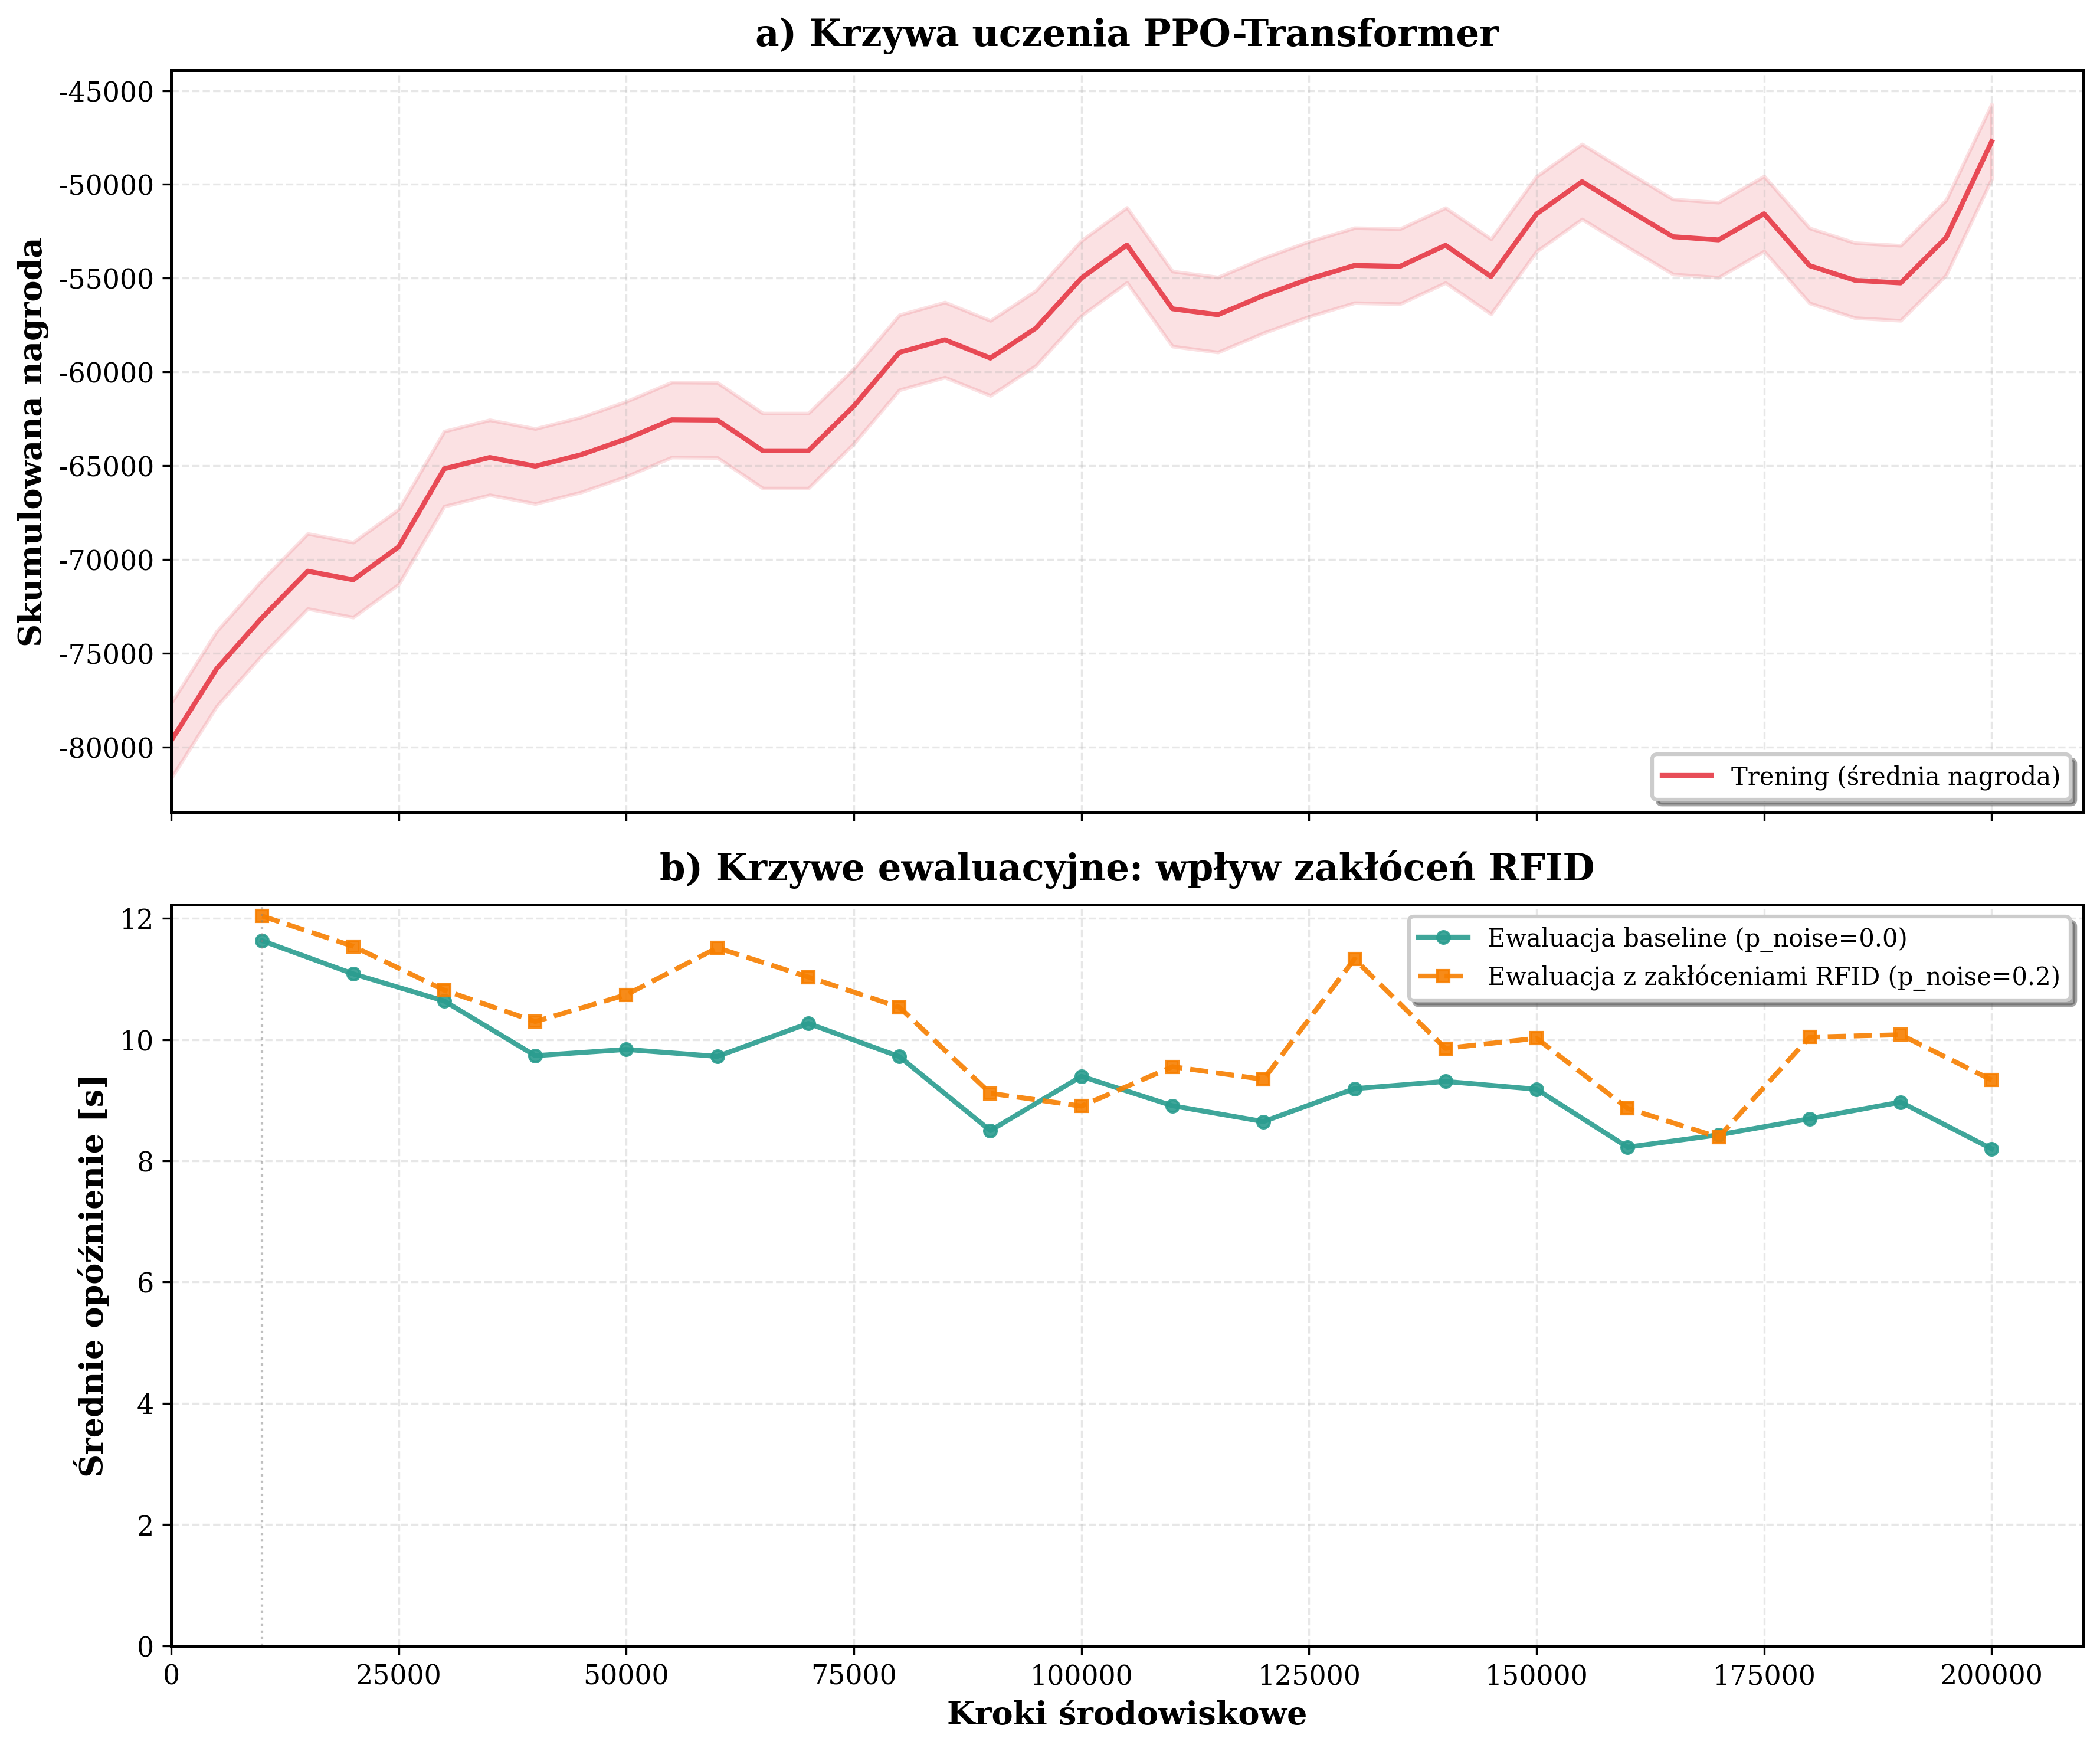
\includegraphics[width=0.9\textwidth]{Rys/R7.png}
\caption{Krzywe uczenia PPO-Transformer oraz krzywe ewaluacyjne dla scenariusza baseline i z zakłóceniami RFID.}
\label{fig:r7}
\end{figure}

\subsection{Rozkłady metryk wydajności}

Rysunek~\ref{fig:r8} przedstawia rozkłady kluczowych metryk wydajności w formie wykresów pudełkowych, porównujące wyniki dla scenariusza baseline oraz scenariusza z zakłóceniami RFID. Analiza rozkładów pozwala na ocenę nie tylko średniej degradacji wydajności, ale także stabilności modelu w warunkach zakłóceń, co jest widoczne w szerokości zakresów międzykwartylowych i występowaniu wartości odstających.

\begin{figure}[H]
\centering
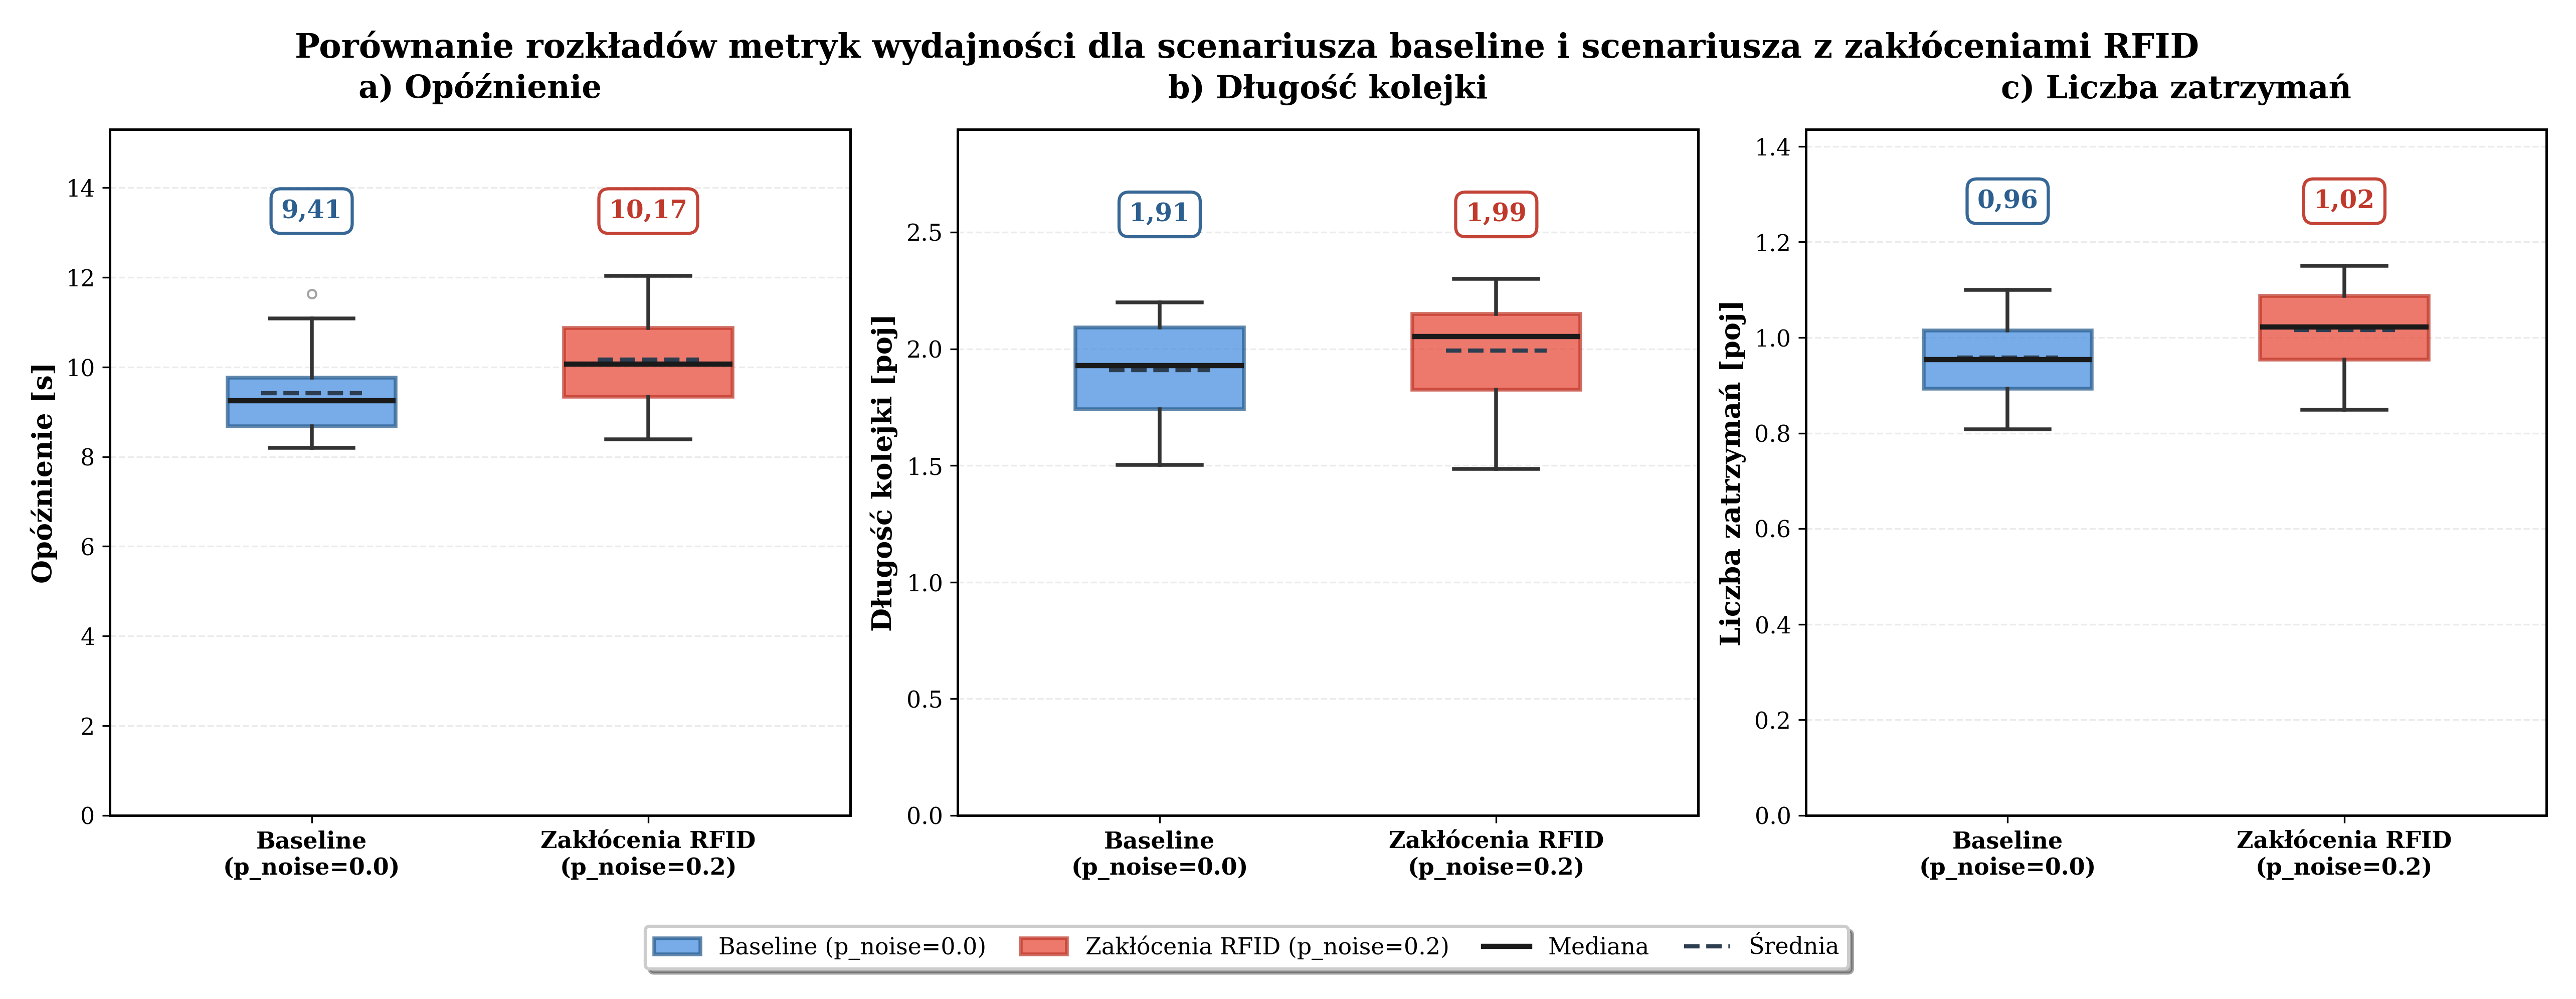
\includegraphics[width=1.0\textwidth]{Rys/R8.png}
\caption{Porównanie rozkładów metryk wydajności dla scenariusza baseline i scenariusza z zakłóceniami RFID: a) Opóźnienie [s]; b) Długość kolejki [poj]; c) Liczba zatrzymań.}
\label{fig:r8}
\end{figure}

\section{Dyskusja}

\subsection{Wydajność w scenariuszu testowym}

Analiza wyników eksperymentalnych w scenariuszu testowym (Tabela~\ref{tab:4}) pozwala na ocenę zdolności generalizacji modelu PPO-Transformer do nowych warunków ruchu. Scenariusz testowy charakteryzuje się asymetrycznym rozkładem natężenia, gdzie kierunek N/S ma wyższe natężenie niż E/W, co stanowi wyzwanie dla modelu wytrenowanego na symetrycznym scenariuszu treningowym. Wyniki wskazują na zdolność modelu do adaptacji do zmiennych warunków ruchu, co jest kluczowe dla praktycznych zastosowań w rzeczywistych systemach ITS, gdzie natężenie ruchu może znacznie różnić się między kierunkami.

\subsection{Minimalizacja długości kolejek}

Analiza wyników eksperymentalnych wykazuje, że model PPO-Transformer skutecznie minimalizuje długość kolejek na skrzyżowaniu poprzez adaptacyjne zarządzanie czasem trwania faz zielonych i wyborem priorytetowego kierunku ruchu. W scenariuszu testowym z asymetrycznym rozkładem natężenia (wyższe natężenie w kierunku N/S), model osiąga średnią długość kolejki wynoszącą 1,62 pojazdów (odchylenie standardowe 0,13), co wskazuje na skuteczne zarządzanie kongestią. Model wykazuje zdolność do dynamicznego dostosowania czasu zielonego światła, co prowadzi do redukcji długości kolejek w porównaniu z tradycyjnymi metodami sterowania o stałej sekwencji faz. Mechanizm self-attention w architekturze Transformer umożliwia modelowi identyfikację wzorców kongestii w sekwencji historycznych obserwacji, co pozwala na predykcyjne podejmowanie decyzji o zmianie fazy przed osiągnięciem krytycznej długości kolejki.

\subsection{Odporność na zakłócenia RFID}

Analiza wrażliwości na zakłócenia RFID (Tabela~\ref{tab:5}) wykazuje odporność modelu PPO-Transformer na częściowe utraty odczytów. Przy symulacji 20\% utraty danych ($p_{\text{noise}} = 0.2$), degradacja wydajności w zakresie minimalizacji długości kolejek pozostaje w akceptowalnych granicach (wzrost długości kolejki o 8,0\% z 1,62 do 1,75 pojazdów), co sugeruje, że model jest zdolny do adaptacji do niekompletnych informacji sensorycznych. Podobnie, opóźnienie wzrasta jedynie o 8,1\% (z 8,12 s do 8,78 s), podczas gdy przepustowość pozostaje praktycznie niezmieniona (spadek o 0,6\%). Ta właściwość ma kluczowe znaczenie dla praktycznych wdrożeń, gdzie awarie detektorów, interferencje elektromagnetyczne lub problemy z infrastrukturą mogą prowadzić do częściowej utraty danych. Model wykorzystuje historyczne obserwacje z okna czasowego $L = 48$ kroków, aby uzupełnić brakujące informacje o bieżącym stanie kolejek.

Mechanizm self-attention w architekturze Transformer prawdopodobnie przyczynia się do tej odporności poprzez zdolność do ważenia znaczenia historycznych obserwacji. Gdy część bieżących odczytów jest utracona, model może wykorzystać informacje z poprzednich kroków czasowych w sekwencji, aby uzupełnić brakujące dane. Dodatkowo, okno czasowe $L = 48$ kroków (odpowiadające 4 minutom historii) zapewnia wystarczający kontekst dla modelu, aby zidentyfikować wzorce ruchu nawet przy częściowej degradacji danych wejściowych.

\subsection{Wpływ zakłóceń na stabilność decyzji i długość kolejek}

Analiza rozkładów metryk wydajności (Rysunek~\ref{fig:r8}) wskazuje na wpływ zakłóceń RFID na stabilność decyzji modelu, szczególnie w kontekście zarządzania długością kolejek. Porównanie zakresów międzykwartylowych między scenariuszem baseline a scenariuszem z zakłóceniami pozwala ocenić, czy degradacja wydajności jest systematyczna czy losowa. W kontekście długości kolejek, węższe zakresy międzykwartylowe w scenariuszu z zakłóceniami mogą wskazywać na bardziej konserwatywne decyzje agenta (dłuższe czasy zielonego światła), podczas gdy szersze zakresy mogą sugerować większą zmienność w odpowiedzi na niepewne dane wejściowe, co może prowadzić do okresowych wzrostów długości kolejek.

\subsection{Ograniczenia i przyszłe kierunki badań}

Niniejsze badanie koncentruje się na pojedynczym skrzyżowaniu i jednym poziomie zakłóceń ($p_{\text{noise}} = 0.2$). Przyszłe badania powinny obejmować analizę wrażliwości dla różnych poziomów zakłóceń (np. $p_{\text{noise}} \in \{0.1, 0.2, 0.3, 0.4\}$), co pozwoliłoby na określenie progu degradacji wydajności. Dodatkowo, warto zbadać wpływ różnych typów zakłóceń, takich jak bursty errors (skupione utraty odczytów w krótkich okresach) versus random errors (losowe utraty rozłożone równomiernie w czasie), na wydajność modelu.

\section{Wnioski}

Niniejsze badanie demonstruje ewolucję systemu sterowania ruchem, przechodząc od fizycznego modelu demonstracyjnego opartego na RFID do zaawansowanego agenta PPO-Transformer w środowisku symulacyjnym SUMO. Wykazano, że na poziomie pojedynczego, izolowanego skrzyżowania -- fundamentalnego scenariusza testowego -- proponowane podejście, zasilane danymi z transponderów, wykazuje zdolność do adaptacji do zmiennych warunków ruchu oraz odporność na częściowe utraty danych sensorycznych.

Kluczowe ustalenia z przeprowadzonych eksperymentów obejmują: (1) zdolność modelu do efektywnej minimalizacji długości kolejek poprzez adaptacyjne zarządzanie czasem trwania faz zielonych i wyborem priorytetowego kierunku ruchu, (2) zdolność do generalizacji do scenariusza testowego z asymetrycznym rozkładem natężenia ruchu, gdzie model skutecznie dostosowuje sterowanie do wyższego natężenia w kierunku N/S, (3) odporność na zakłócenia RFID przy poziomie $p_{\text{noise}} = 0.2$, gdzie degradacja wydajności w zakresie minimalizacji kolejek pozostaje w akceptowalnych granicach, oraz (4) stabilność decyzji sterujących nawet w warunkach niekompletnych danych wejściowych, co jest kluczowe dla praktycznych wdrożeń w rzeczywistych systemach ITS.

Kluczowe wyzwanie zidentyfikowane w niniejszej pracy pozostaje kwestią skalowalności i tendencji do optymalizacji lokalnej, która jest niewystarczająca na skalę sieci miejskiej. Ta złożoność jest dodatkowo komplikowana przez rosnącą heterogeniczność floty, obejmującą pojazdy elektryczne i autonomiczne, a także konieczność zarządzania dynamicznymi priorytetami (TSP dla transportu publicznego, EVP dla pojazdów uprzywilejowanych) oraz wymogami regulacyjnymi, takimi jak Strefy Czystego Transportu. Badanie wskazuje, że przyszłe systemy muszą opierać się na fuzji danych z komplementarnych źródeł, gdzie systemy wizyjne szacują kolejki, podczas gdy technologia RFID zapewnia weryfikację tożsamości dla konkretnych pojazdów.

Na podstawie tych wniosków, przyszłe badania będą koncentrować się na przejściu od modelu jednoagentowego do wielopoziomowej, warstwowej architektury zarządzania dla całej sieci miejskiej, zgodnie z koncepcją przedstawioną na Rysunku~\ref{fig:r9}. To podejście, zgodne z rekomendacjami dotyczącymi Multi-Agent RL (MARL) sformułowanymi w przeglądzie literatury, zakłada dekompozycję problemu na poziomy hierarchiczne. Na najniższym poziomie, poziomie skrzyżowania, będą działać autonomiczne agenty (takie jak PPO-Transformer), optymalizujące lokalny przepływ na podstawie fuzji danych. Poziom pośredni, sektor miasta, będzie zarządzany przez modele nadzorcze, których zadaniem nie jest bezpośrednie sterowanie sygnałami, ale wykrywanie wzorców ruchu na skalę dzielnicy (np. fale ruchu) i ustawianie celów dla podległych lokalnych agentów. To rozwiązuje problem czysto lokalnej optymalizacji i umożliwia koordynację, zgodną z obiecującymi wynikami dla Federated Learning.

\begin{figure}[H]
\centering
\includegraphics[width=0.8\textwidth]{Rys/R9.png}
\caption{Koncepcja hierarchicznej (warstwowej) architektury sterowania siecią miejską.}
\label{fig:r9}
\end{figure}

Na najwyższym poziomie, poziomie miasta, model sterowania głównego będzie odpowiedzialny za globalną optymalizację, równoważenie przepływu między sektorami i realizację celów optymalizacji wielokryterialnej, obejmującej nie tylko płynność ruchu, ale także emisje CO$_2$ i bezpieczeństwo. Dalsze badania będą również obejmować rozwój metod Explainable AI (XAI) w celu poprawy zaufania do systemu, integrację z komunikacją V2X oraz walidację algorytmów w rzeczywistych warunkach miejskich, co zostało zidentyfikowane jako kluczowy kierunek badawczy.

\begin{thebibliography}{99}

\bibitem{ref1}
Qadri SSSM, Gökçe MA, Öner E. State-of-art review of traffic signal control methods: challenges and opportunities. Eur Transp Res Rev. 2020;12(1):55. doi: 10.1186/s12544-020-00439-1

\bibitem{ref2}
Michailidis P, Michailidis I, Lazaridis CR, Kosmatopoulos E. Traffic Signal Control via Reinforcement Learning: A Review on Applications and Innovations. Infrastructures. 2025;10(5):114. doi: 10.3390/infrastructures10050114

\bibitem{ref3}
Pawłowicz B, Trybus B, Salach M, Jankowski-Mihułowicz P. Dynamic RFID Identification in Urban Traffic Management Systems. Sensors. 2020;20(15):4225. doi: 10.3390/s20154225

\bibitem{ref4}
Lopez PA, Behrisch M, Bieker-Walz L, Erdmann J, Flötteröd Y, Hilbrich R, et al. Microscopic Traffic Simulation using SUMO. IEEE Xplore. 2018. p. 2575-82. doi: 10.1109/ITSC.2018.8569938

\bibitem{ref5}
Schulman J, Wolski F, Dhariwal P, Radford A, Klimov O. ``Proximal Policy Optimization Algorithms''. In: arXiv preprint arXiv:1707.06347 (2017). doi: 10.48550/arXiv.1707.06347

\bibitem{ref6}
Vaswani A, Shazeer N, Parmar N, Uszkoreit J, Jones L, Gomez AN, et al. ``Attention Is All You Need''. In: Advances in Neural Information Processing Systems 30 (NIPS 2017). 2017, pp. 5998-6008. doi: 10.48550/arXiv.1706.03762

\bibitem{ref7}
Federal Highway Administration. Traffic Analysis Tools Program: Traffic Analysis Toolbox, Volume II: Decision Support Methodology for Selecting Traffic Analysis Tools. U.S. Department of Transportation, 2004. (Accessed: 18.11.2025). url: https://ops.fhwa.dot.gov

\bibitem{ref8}
SUMO Documentation. routeSampler.py - SUMO Documentation. 2023. (Accessed: 18.11.2025). url: https://sumo.dlr.de/docs/Tools/Routes.html

\bibitem{ref9}
Federal Highway Administration. Traffic Analysis Tools Program: Guidebook on Traffic Signal Control Algorithms and Applications. U.S. Department of Transportation, 2010. (Accessed: 18.11.2025). url: https://ops.fhwa.dot.gov

\bibitem{ref10}
Yavuz MN, Özen H. Calibration of microscopic traffic simulation of urban road network including mini-roundabouts and unsignalized intersection using open-source simulation tool. Sci J Silesian Univ Technol Ser Transp. 2024;122:305-18. doi: 10.20858/sjsutst.2024.122.17

\bibitem{ref11}
Islam I, Li W, Li S, Heaslip K. Heterogeneous Mixed Traffic Control and Coordination. arXiv (Cornell University). 2024 Sep 18. doi: 10.48550/arXiv.2409.12330

\bibitem{ref12}
Transportation Research Board. Highway Capacity Manual (HCM). Washington, D. C.: Transportation Research Board, 2010. (Accessed: 18.11.2025). url: https://onlinepubs.trb.org/Onlinepubs/sr/sr209/209.pdf

\bibitem{ref13}
Dion F, Rakha H, Kang Y-S. Comparison of delay estimates at under-saturated and over-saturated pre-timed signalized intersections. Transp Res Part B Methodol. 2004;38(2):99-122. doi: 10.1016/S0191-2615(03)00003-1

\bibitem{ref14}
Huang L, Qu X. Improving traffic signal control operations using proximal policy optimization. IET Intell Transp Syst. 2023;17(3). doi: 10.1049/itr2.12286

\bibitem{ref15}
Stęchły A, Pawłowicz B, Siwiec K, Drzał J, Kosior A. Top-level smart city traffic management system with radio frequency identification - based road event detection. Advances in Science and Technology Research Journal. 2025;19(11):429-441. doi: 10.12913/22998624/209674

\bibitem{ref25}
% Placeholder for reference 25 - add actual citation if needed

\end{thebibliography}

\end{document}

